\documentclass[10pt]{beamer}
\usetheme{PaloAlto}

\usepackage{caption}
\usepackage{graphicx}
\usepackage{amsmath}
\usepackage{amssymb}
\usepackage{hyperref}

\title{General Neural Network Class}
\institute{Indian Institute of Technology Bombay
}
\author{M Suriya Kumar \& Siddharth Swarnkar, Group : 19}
\date{}

\begin{document}

\begin{frame}[plain]
\maketitle
\end{frame}

\section{Description of Project}
\begin{frame}
\frametitle{About Neural Network}
\begin{block}{What is neural network ?}
In machine learning and cognitive science, artificial neural networks (ANNs) are a family
of models inspired by biological neural networks (the central nervous systems of
animals) which are used to estimate or approximate functions that can depend on a 
large number of inputs and are generally unknown.

\textbf{Applications : } Image processing, Self driving cars, Stock market prediction 
\end{block}

\begin{figure}
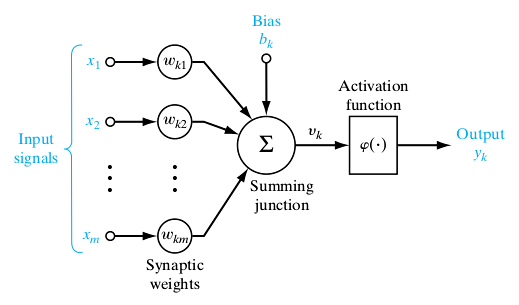
\includegraphics[scale=0.26]{nnnode.png}
\caption{The McCullogh-Pitts model of a neuron}
\end{figure}
\end{frame}


\begin{frame}
\frametitle{What we would like to do?}
\begin{itemize}
\item{Model the neural network using OOPs concept.}
\item{Given the data and details about the neural network, we would train the network
and return the synaptic weights}
\item{Give various option for activation function and optimization techniques}
\item{Develop numerical optimization techniques, esp. :}
	\begin{itemize}
	\item{Gradient descent}
	\item{Conjugate gradient descent}
	\end{itemize}
\item{Develop various activation function and efficient way to calculate associated 
cost function and partial derivatives of the cost function, esp. :}
	\begin{itemize}
	\item{Sigmoid}
	\item{Linear}
	\item{ReLU}
	\end{itemize}	
\end{itemize}
\end{frame}

\section{Approach}

\begin{frame}
\frametitle{Approach}
\begin{itemize}
\item{ \textbf{Step 1 : } Develop low level helper functions}
\item{ \textbf{Step 2 : } Develop test cases to check optimization functions' stability and correctness/accuracy}
\item{ \textbf{Step 3 : } Develop optimization functions and optimize code for better perfomance}
\item{ \textbf{Step 4 : } Create class node and associated activation functions}
\item{ \textbf{Step 5 : } Create class neural\_network}
\item{ \textbf{Step 6 : } Develop efficient way to compute cost function for different activation function}
\item{ \textbf{Step 7 : } Develop training algorithm and optimize code for optimal performance}
\item{ \textbf{Step 8 : } Run the model for well-known examples and compare the results}
\end{itemize}
\end{frame}

\begin{frame}
\frametitle{Status}
\begin{block}{Accomplished tasks}
\begin{itemize}
\item{Efficient way to optimize a given function using both
gradient descent and conjugate gradient descent}
\item{Tests to check for stability and correctness of the solution}
\item{Helper functions for various maths associated tasks}
\end{itemize}
\end{block}

\begin{alertblock}{To be done..}
\begin{itemize}
\item{Create class node which describe the behaviour of the neuron}
\item{Create class neural network to characterize the network}
\item{Develop efficient training algorithm to find the necessary parameters}
\item{Develop cost functions for different activation function}
\end{itemize}
\end{alertblock}
\end{frame}

\section{If time permits..}
\begin{frame}
If time permits...
\begin{itemize}
\item{Create visualization utilities for learning purposes}
\item{Create GUI for easy input and visualization}
\end{itemize}
\vspace{5cm}
\textbf{github repo link :} 
\url{https://github.com/siddharthswarnkar/generalNNClass}

\end{frame} 
\end{document}

